\chapter{Requisitos y Análisis del problema}

\section{Requisitos funcionales}
Un requisito funcional es una declaración que describe una función o característica específica que debe cumplir un sistema o software, estos requisitos definen qué debe hacer el sistema y cómo debe comportarse en términos de funcionalidad. En la Tabla~\ref{tab:requisitosfunionales} se podrán ver los requisitos funcionales del sistema.
\begin{table}[htbp]

\begin{tabular}{p{2cm} p{12cm}}
RF-01 & El sistema deberá implementar un dispositivo hardware, compuesto por un dispositivo Raspberry-Pi con sensores conectados, para la toma de medidas. \\ \\
RF-02 & El sistema deberá contar con un servidor Erlang donde los usuarios puedan interactuar.\\ \\
RF-03 &  El sistema deberá tomar medidas de distancia mediante un sensor de ultrasonidos.\\ \\
RF-04 &  El sistema deberá tomar medidas de cabeceo con respecto al campo magnético mediante un sensor magnetómetro.\\ \\
RF-05 &  El sistema deberá tomar como mínimo 10 medidas por segundo para hacer la demostración en tiempo real.\\ \\
RF-06 &  El sistema deberá almacenar los datos obtenidos en archivos de texto para su posterior análisis.\\ \\
RF-07 &  El servidor deberá poder comunicarse con la placa R-Pi para lanzar la lectura de los sensores.\\ \\
RF-08 & El sistema deberá poder comunicarse con el servidor para poder los archivos con la información de las medidas.\\ \\
RF-09 & El servidor deberá permitir al usuario consultar la descripción de los sensores. \\ \\
RF-10 & El servidor deberá permitir al usuario interactuar mediante una arquitectura API REST. \\ \\
RF-11 & El servidor deberá permitir al usuario visualizar los archivos de datos obtenidos por los sensores. \\ \\
RF-12 & El servidor deberá permitir al usuario modificar los parámetros de lanzamiento de los sensores. \\ \\
RF-12 & El servidor deberá ofrecer un manual de uso de la interfaz al usuario. \\ \\



\end{tabular}
\label{tab:requisitosfunionales}
\caption{Requisitos Funcionales}
\end{table}

\section{Requisitos no funcionales}

Se entiende como requisito no funcional, dentro del ámbito de la ingeniería del software, a un requisito que describe una cualidad o restricción que debe cumplir el sistema en términos de rendimiento, seguridad, usabilidad, mantenibilidad u otras características no directamente relacionadas con la funcionalidad específica. Por lo tanto, se trata de las restricciones o condiciones impuestas por el usuario que ordena desarrollar este sistema.
En la Tabla~\ref{tab:requisitosnofunionales} se enumeran los requisitos no funcionales del sistema.
\begin{table}[htbp]

\begin{tabular}{p{2cm} p{12cm}}
RNF-01 & El sistema deberá utilizar un dispositivo de medición de datos diseñado sobre Raspberry-Pi.\\ \\
RNF-02 & El sistema deberá utilizar un servidor creado con lenguaje Erlang OTP.\\ \\
RNF-03 & El servidor deberá ser eficiente en el procesamiento de solicitudes y proporcionar una respuesta rápida a los usuarios.\\ \\
RNF-04 &  El sistema debe ser compatible con diferentes plataformas y navegadores web, asegurando una amplia accesibilidad para los usuarios.\\ \\
RNF-05 & El sistema deberá ser fácilmente usable e intuitivo una vez leído el manual de funcionamiento.\\ \\
RNF-06 &  El sistema deberá ser confiable, asegurando la respuesta esperada.\\ \\
RNF-07 & El sistema deberá almacenar la información recogida durante el tiempo de muestreo. \\ \\
RNF-08 &  El sistema debe estar disponible y operativo la mayor parte del tiempo, minimizando los períodos de inactividad.\\ \\
RNF-09 & El sistema debe garantizar la seguridad de los datos transmitidos y almacenados..\\ \\
RNF-10 & El código del sistema debe ser modular, legible y fácilmente mantenible para facilitar futuras actualizaciones y correcciones.\\ \\
RNF-11 & El sistema estar diseñado para ser fácilmente escalable, de esta manera pueden añadirse más sensores con posterioridad.\\ \\



\end{tabular}
\label{tab:requisitosnofunionales}
\caption{Requisitos No Funcionales}
\end{table}

\newpage

\section{Diagramas SysML del modelo}

\subsection{Diagrama de paquetes del modelo}

En el diagrama presentado en la Figura~\ref{fig:diagramaPaquetes}, se muestra el Diagrama de Paquetes del modelo del sistema que incluye aquellos modelos que se han elaborado para mostrar el sistema y los requisitos del mismo, este diagrama podría ser ampliable e incluir más elementos pero se ha decidido mostrar únicamente aquellos que realmente muestran información importante para la realización del proyecto. Este diagrama incluye:

Diagramas de casos de uso y secuencia para mostrar el comportamiento y dos diagramas de descripción de bloques que muestran la descripción de la estructura del sistema a alto nivel. En el caso de las pruebas no se han realizado diagramas pero se incluye su descripción textual en lo sucesivo.


\begin{figure}[h!]
\centering
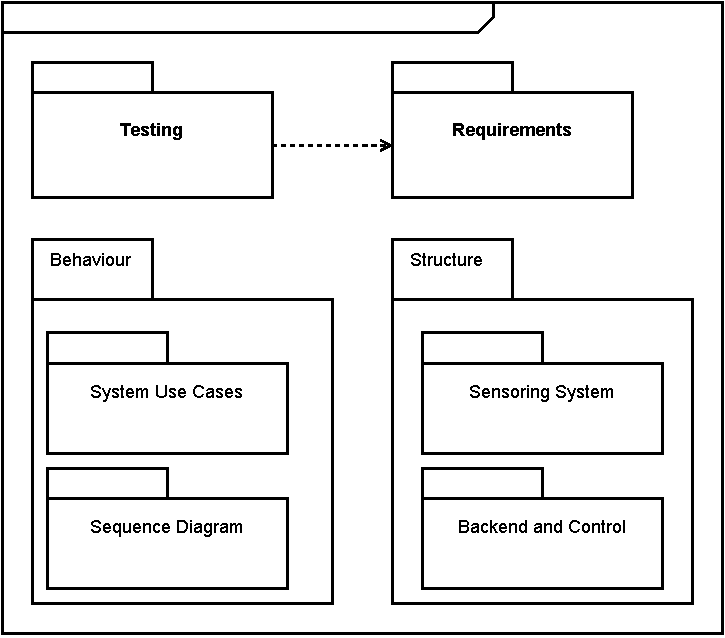
\includegraphics{images/diagramaDePaquetes.pdf}
\caption{Diagrama de paquetes}%
\label{fig:diagramaPaquetes}
\end{figure}

\subsection{Diagrama de casos de uso}

Un diagrama de casos de uso es una herramienta utilizada en el análisis y diseño de sistemas para representar las interacciones entre los actores (usuarios o sistemas externos) y un sistema en particular. Proporciona una visión general de las funciones que el sistema ofrece y cómo se relaciona con los usuarios.

En un diagrama de casos de uso, los casos de uso se representan como elipses y los actores como figuras externas al sistema. Las flechas indican las interacciones entre los actores y los casos de uso, mostrando qué funciones realiza el sistema en respuesta a las acciones de los usuarios. El objetivo principal de un diagrama de casos de uso es capturar los requisitos funcionales del sistema y comprender cómo los usuarios interactúan con él. Ayuda a identificar las diversas formas en que los usuarios pueden utilizar el sistema y los escenarios en los que se involucran.

En el caso de nuestro proyecto contamos con dos actores: el administrador y el usuario.
\begin{itemize}
    \item \textbf{Administrador}: Encargado de configurar el servidor, disponiendo de la posibilidad de añadir o eliminar sensores al sistema, a su vez puede realizar las mismas actividades que realiza un usuario.
    \item \textbf{Usuario}: Puede acceder a la interfaz web para: lanzar la lectura de los sensores, ver el manual de uso, ver las especificaciones de los sensores o ver los datos obtenidos por los mismos.
\end{itemize}

Puede observarse el diagrama de casos de uso en la Figura~\ref{fig:usecases}


\begin{figure}[h!]
\centering
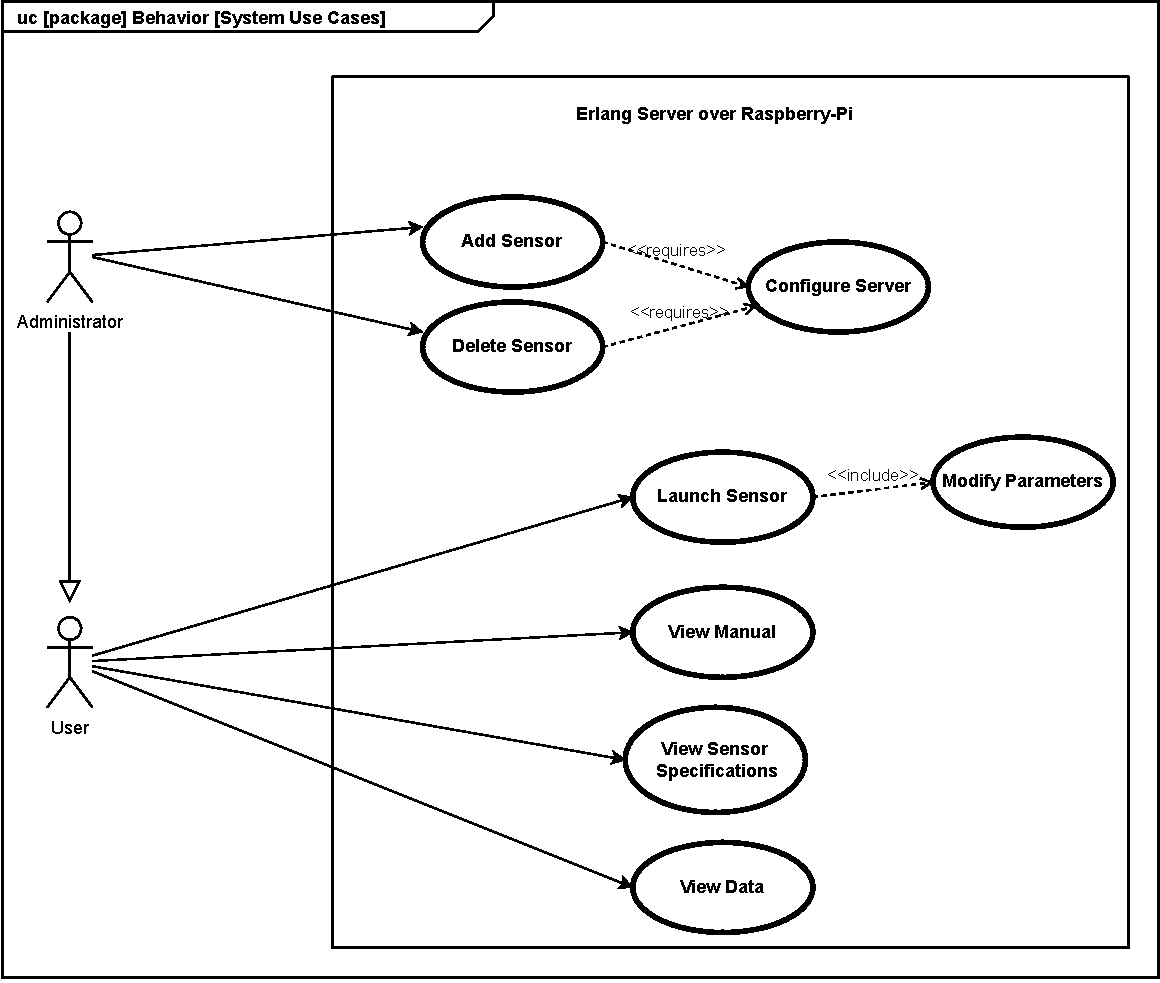
\includegraphics[width=\textwidth]{images/casosUso.pdf}
\caption{Diagrama de Casos de Uso del sistema}%
\label{fig:usecases}
\end{figure}

\clearpage

\subsection{Diagrama de secuencia}

En el segundo diagrama de comportamiento del sistema, el diagrama de secuencia observado en la Figura~\ref{fig:diagramaSecuencia}, se pueden identificar varios pasos clave:

\begin{figure}[t]
\centering
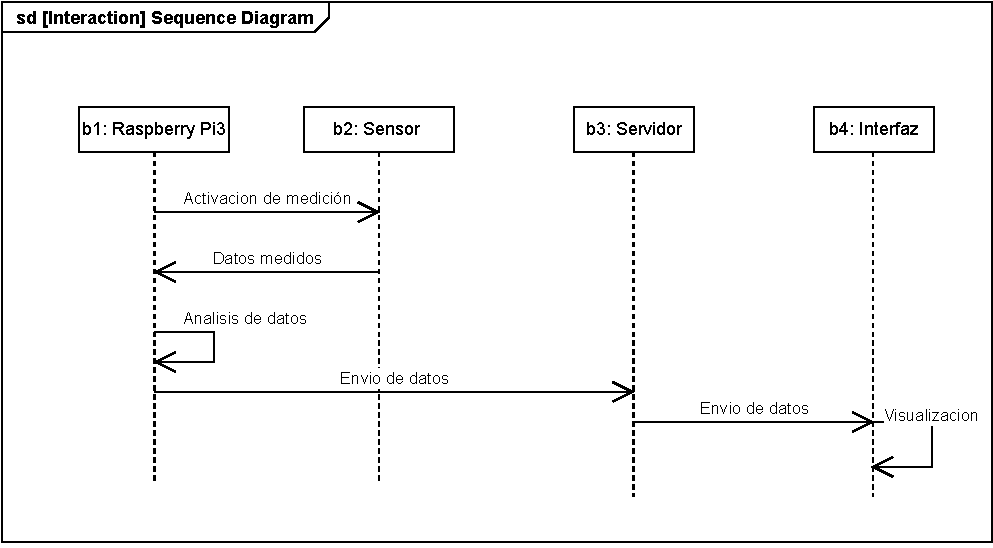
\includegraphics[width=\textwidth]{images/diagramaSecuencia.pdf}
\caption{Diagrama de Secuencia}%
\label{fig:diagramaSecuencia}
\end{figure}



\begin{enumerate}
\item Activar medición: Se activa el sensor para que comience a medir los datos.

\item Datos medidos: El sensor envía los datos medidos a la placa R-Pi a través de un protocolo de comunicación adecuado (como puede ser I2C).

\item Analizar datos en C: La placa R-Pi recibe los datos del sensor, los procesa a través de un código en C que los analiza y transforma en un formato adecuado para su almacenamiento y posterior envío al servidor.

\item Datos analizados: Una vez que el código en C ha analizado los datos, los envía de vuelta a la placa R-Pi en un formato adecuado para su almacenamiento.

\item Guardar en archivo: Cuando la placa R-Pi ha recibido los datos analizados, los guarda en un archivo local en la placa de desarrollo para su posterior envío al servidor.

\item Enviar archivo: la placa R-Pi envía el archivo con los datos analizados al servidor a través de una conexión adecuada (como puede ser una conexión por Internet).

\item Recibir archivo: el servidor recibe el archivo con los datos analizados enviado por la placa R-Pi.

\item Analizar archivo: el servidor analiza los datos recibidos en el archivo y genera los resultados.

\item Resultados: el servidor envía los resultados a la interfaz para que sean visualizados por el usuario.
\end{enumerate}


\subsection{Diagrama de bloques: Sensoring System}

El diagrama de bloques del sistema se encuentra disponible en la Figura~\ref{fig:diagramaBloques}, en él pueden observarse los objetos principales del sistema y como estos se comunican entre sí. El sensor es el dispositivo encargado de recolectar los datos, estos datos se transmiten al Web Service a través de un protocolo I2C de conexión el cual puede almacenar hasta 7 dispositivos, de ahí su cardinalidad.


\begin{figure}[h!]
\centering
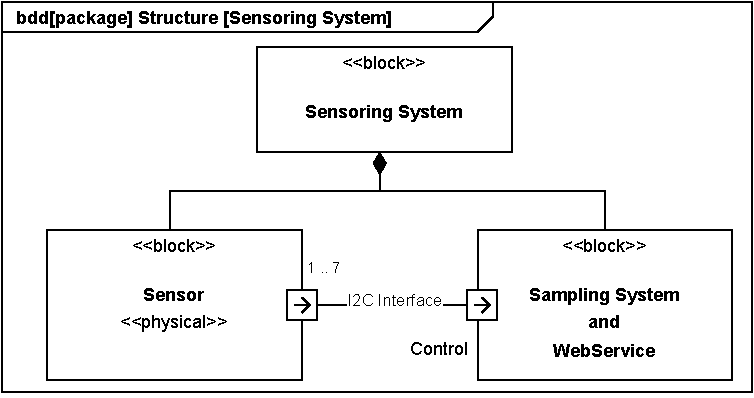
\includegraphics[scale=1.2]{images/bloques.pdf}
\caption{Diagrama de bloques: Sensoring System.}%
\label{fig:diagramaBloques}

\end{figure}


\subsection{Diagrama de bloques: Control y Backend}


En la Figura~\ref{fig:diagramaControl} se puede observar el otro diagrama de bloques que describe el Backend y Control del sistema, en él puede observarse la comunicación entre los diferentes componentes y los protocolos utilizados, a su vez puede verse cuál de ellos tiene el control sobre la comunicación.

\begin{figure}[h!]
\centering
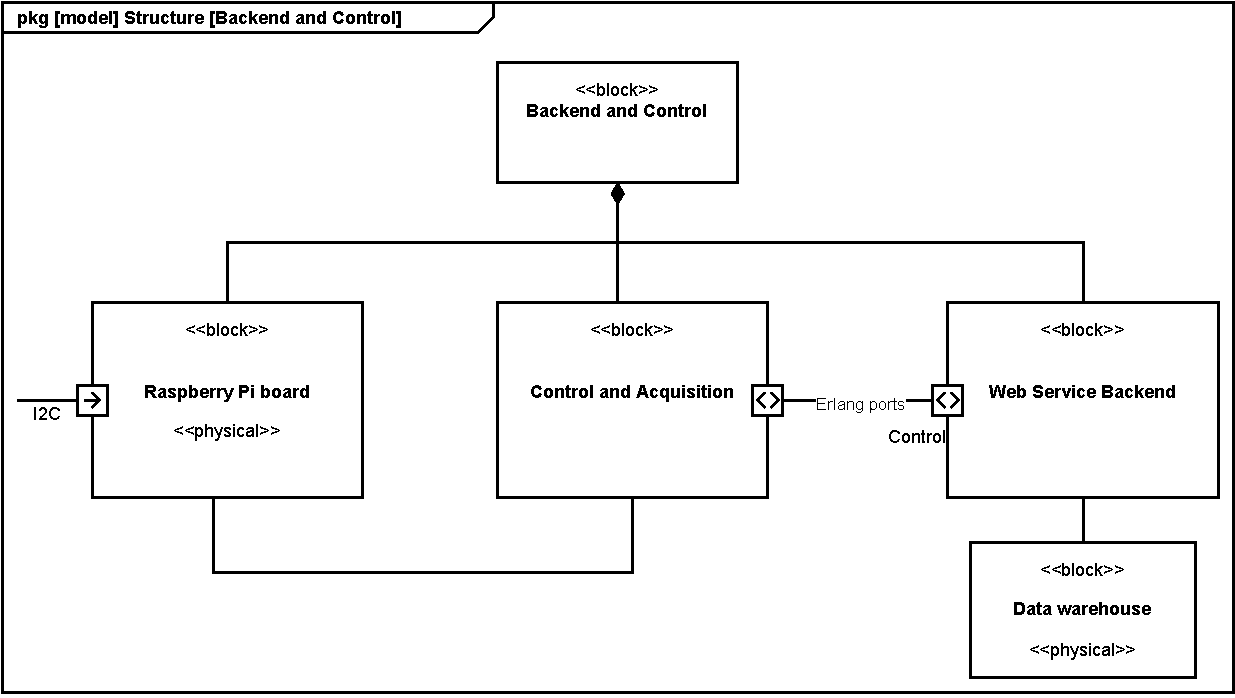
\includegraphics[width=\textwidth]{images/model.pdf}
\caption{Diagrama de Bloques: Control y Backend.}%
\label{fig:diagramaControl}

\end{figure}


